\documentclass[11pt]{article}

\usepackage{a4wide}
\usepackage[utf8]{inputenc}
\usepackage[russian]{babel}
\usepackage{graphicx}
\usepackage{amsmath}
\usepackage{amsthm}
\usepackage{amssymb}

\newtheorem{theorem}{Теорема}
\newtheorem{definition}{Определение}
\newtheorem{proposition}{Утверждение}

\newcommand*{\hm}[1]{#1\nobreak\discretionary{}{\hbox{$\mathsurround=0pt #1$}}{}}
\newcommand\abs[1]{\left\lvert#1\right\rvert}
\newcommand{\scalar}[2]{\left<#1,#2\right>}
\newcommand{\norm}[1]{\left\lVert #1 \right\lVert}
\newcommand{\const}{\ensuremath{\operatorname{const}}}
\newcommand{\sgn}{\ensuremath{\operatorname{sgn}}}
\newcommand{\Real}{\ensuremath{\operatorname{Re}}}
\renewcommand{\d}[1]{\ensuremath{\operatorname{d}\!{#1}}}
\DeclareMathOperator{\Tr}{Tr}
%\DeclareMathOperator{\det}{det}

\begin{document}
\thispagestyle{empty}

\begin{center}
\ \vspace{-3cm} \newline
\includegraphics[width=0.5\textwidth]{msu.eps}\\
{\scshape Московский государственный университет имени М.~В.~Ломоносова}\\
Факультет вычислительной математики и кибернетики\\
Кафедра системного анализа

\vfill

{\LARGE Курсовая работа} \newline
%\vspace{1cm}
{\Huge\bfseries Изучение динамических систем с непрерывным временем}
\end{center}

\vspace{1cm}
\begin{flushright}
\large
\textit{Студент 315 группы}\\
В.~С.~Терёшин\\
\vspace{5mm}
\textit{Преподаватель}\\
д.ф.-м.н., профессор А.~С.~Братусь
\end{flushright}

\vfill
\begin{center}
Москва, 2014
\end{center}
\pagebreak
\tableofcontents
\pagebreak
\section{Постановка задачи}
Дана непрерывная динамическая система, описывающая некую модель типа хищник-жертва:
\begin{gather}
\left\{ \begin{aligned}
\dot{x} = \frac{ax^2}{N + x}\left( \frac{K - x}{K} \right) - bxy, \\
\dot{y} = -cy + dxy,
\end{aligned} \right. %\label{eq:1}
\end{gather}
где $x, y \geqslant 0$, а $a, b, c, d, N, K > 0$. Необходимо выполнить:
\begin{enumerate}
\item
Дать биологическую интерпретацию системе;
\item
Ввести безразмерные переменные, максимально уменьшив число входящих параметров;
\item
Найти неподвижные точки системы и исследовать их характер;
\item
Построить параметрический портрет системы;
\item
Для каждой области параметрического портрета построить фазовый портрет;
\item
Если в системе возникает бифуркация Андронова-Хопфа, то вычислить первое Ляпуновское число;
\item
Дать биологическое объяснение поведению системы при разных значениях параметров.
\end{enumerate}

\section{Биологическая интерпретация системы}

Эта система является моделью хищник-жертва, где $x$ --- численность попопуляции жертв, а $y$ --- хищников. Жертвы в данной системе являются автотрофами, то есть питаются за счёт некоторого биологического ресурса за пределами данной системы, а хищники являются гетеротрофами и питаются жертвами. При отсутствии жертв ($x = 0$) они очень быстро вымрут в силу уравнения $\dot{y} = -cy$. Отсюда видно, что параметр $c$ обозначает скорость вымирания хищников при отсутствии жертв, а параметр $d$ --- какое влияние оказывают жертвы на рост популяции хищников. Параметр $a$ обозначает скорость размножения жертв.

Параметр $K$ обозначает биологическую ёмкость рассматриваемой системы. При достижении жертвами численности $K$ их размножение прекращается. Параметр $N$ характеризует резкое уменьшение скорости роста популяции при её численности $x \ll N$. $b$ --- скорость истребления жетрв хищниками. Кроме того, если жертв не очень много, то хищники съедают их со скоростью, зависящей и от их численности, и от численности жертв. Если же число жертв привосходит число хищников, то скорость поедания зависит только от числа хищников.

\section{Ввод безразмерных параметров}

Пусть $x = Au$, $y = Bv$, $t = T\tau$. Тогда система 1 принимает вид:
\begin{gather}
\left\{ \begin{aligned}
\frac{A}{T}\dot{u} = \frac{aA^2u^2}{N + Au}\left( \frac{K - Au}{K} \right) - bABuv, \\
\frac{B}{T}\dot{v} = -cBv + dABuv.
\end{aligned} \right. \\ %\label{eq:2}
\left\{ \begin{aligned}
\dot{u} = \frac{aTu^2}{\frac{N}{A} + u}\left( 1 - \frac{A}{K}u \right) - bTBuv, \\
\dot{v} = -cBv + dTBuv.
\end{aligned} \right. %\label{eq:3}
\end{gather}

Положим $bTB = 1$, $dTA = 1$, $\frac{N}{A} = 1$. Отсюда получаем:
\begin{gather}
\left\{ \begin{aligned}
A = N, \\
B = \frac{dN}{b}, \\
T = \frac{1}{dN}.
\end{aligned} \right.
\end{gather}

Введём обозначения $\alpha = aT$, $\beta = \frac{B}{K}$, $\gamma = cT$ и получим систему:
\begin{gather}
\left\{ \begin{aligned}
\dot{u} = \frac{\alpha u^2}{1 + u}(1 - \beta u) - uv, \\
\dot{v} = -\gamma v + uv.
\end{aligned} \right.
\end{gather}

Зафиксируем $\beta = 1$, вернёмся к прежним обозначениям и будем исследовать систему:
\begin{gather}
\left\{ \begin{aligned}
\dot{x} = \frac{\alpha x^2}{1 + x}(1 - x) - xy, \\
\dot{y} = -\gamma y + xy.
\end{aligned} \right.
\end{gather}

\section{Исследование непожвижных точек}
\begin{theorem}[Ляпунова-Пуанкаре]
Пусть $u^*$ --- положение равновесия, а $J(u)$ --- матрица Якоби исследуемой динамической системы. Тогда если вещественные части всех собственных значений матрицы $J(u^*)$ отрицательны, тогда положение равновесия $u^*$ ассимптотически устойчиво, а если есть хотя бы одно собственное значение с положительной вещественной частью, то положение равновесия $u^*$ неустойчиво.
\end{theorem}

Для нахождения неподвижных точек режим систему:
\begin{gather}
\left\{ \begin{aligned}
\frac{\alpha x^2}{1 + x}(1 - x) - xy = 0, \\
-\gamma y + xy = 0.
\end{aligned} \right.
\end{gather}

Точки $O(0, 0)$ и $P(1, 0)$, очевидно, являются неподвижными для любых значений параметров. При $\gamma \in (0, 1)$ также существует неподвижная точка $Q\left(\gamma, \frac{\alpha\gamma(1 - \gamma)}{1 + \gamma}\right)$.

Матрица Якоби для данной системы:
$$
J(x, y) = \left[ \begin{array}{ccc}
-2\alpha x \frac{x^2 + x - 1}{(x+1)^2} & -x \\[0.5em]
y & x - \gamma
\end{array} \right]
$$

\subsection{Точка $O(0, 0)$}

Подставим в матрицу Якоби неподвижную точку $O(0, 0)$:
$$
J(0, 0) = \left[ \begin{array}{ccc}
0 & 0 \\[0.5em]
0 & -\gamma
\end{array} \right]
$$

$\lambda_1 = \lambda_2 = 0$, а значит, в данном случае мы не можем применить теорему Ляпунова--Пуанкаре для анализа этой неподвижной точки.

\subsection{Точка $P(1, 0)$}

Подставим в матрицу Якоби неподвижную точку $P(1, 0)$:
$$
J(1, 0) = \left[ \begin{array}{ccc}
-\frac{\alpha}{2} & 0 \\[0.5em]
0 & 1 - \gamma
\end{array} \right]
$$

В данном случае получаем собственные значения $\lambda_1 = -\frac{\alpha}{2}$ и $\lambda_2 = 1 - \gamma$. При этом $\lambda_1 < 0$ при любых допустимых значениях параметра. Таким образом, характер неподвижной точки $P(1, 0)$ зависит только от $\lambda_2$:
\begin{enumerate}
\item
$\gamma \in (0, 1) \Rightarrow \lambda_2 > 0$ --- в этом случае точка $P$ является седлом.
\item
$\gamma > 1 \Rightarrow \lambda_2 < 0$ --- в этом случае точка $P$ является устойчивым узлом.
\item
$\gamma = 0 \Rightarrow \lambda_2 = 0$ --- в этом случае происходит бифуркация типа седло-узел.
\end{enumerate}

\subsection{Точка $Q\left(\gamma, \frac{\alpha\gamma(1 - \gamma)}{1 + \gamma}\right)$}

Матрица Якоби в точке $Q$:
$$
J(Q) = \left[ \begin{array}{ccc}
\frac{\alpha\gamma(-\gamma^2 - 2\gamma + 1)}{(\gamma + 1)^2} & -\gamma \\[0.5em]
\frac{\alpha\gamma(1 - \gamma)}{1 + \gamma} & 0
\end{array} \right]
$$

Рассмотрим след и определитель получившейся матрицы:
\begin{gather}
\Tr J = -\frac{\alpha\gamma(\gamma^2 + 2\gamma - 1)}{(\gamma + 1)^2}, \notag \\
\det J = \frac{\alpha\gamma^2(1 - \gamma)}{1 + \gamma}, \notag \\
\lambda_{1,2} = \frac{1}{2}\left( \Tr J \pm \sqrt{(\Tr J)^2 - 4 \det J} \right). \notag
\end{gather}

Исследуем знак подкоренного выражения:
\begin{gather}
D = (\Tr J)^2 - 4 \det J = \frac{\alpha^2\gamma^2}{\gamma + 1}^3(\gamma^2 + 2\gamma - 1)^2 - \frac{4\alpha\gamma^2(1 - \gamma)}{1 + \gamma} = \notag \\
= \frac{\alpha\gamma^2}{\gamma + 1}\left( \alpha\frac{(\gamma^2 + 2\gamma - 1)^2}{(\gamma + 1)^3} - 4(1 - \gamma) \right), \notag \\
D > 0 \Rightarrow \alpha\frac{(\gamma^2 + 2\gamma - 1)^2}{(\gamma + 1)^3} - 4(1 - \gamma > 0) \Rightarrow \alpha > \frac{4(1 - \gamma)(\gamma + 1)^3}{(\gamma^2 + 2\gamma - 1)^2}, \notag \\
D < 0 \Rightarrow \alpha < \frac{4(1 - \gamma)(\gamma + 1)^3}{(\gamma^2 + 2\gamma - 1)^2}. \notag
\end{gather}

Исследуем знак $\Tr J$. Так как параметры положительны, то знак зависит только от знака выражения $\gamma^2 + 2\gamma - 1$. Значит, $\Tr J > 0$ при $\gamma \in (0, -1 + \sqrt{2})$ и $\Tr J < 0$ если $\gamma \in (-1 + \sqrt{2}, 1)$.

Отметим, что при $\gamma \in (0, 1)$ выполнено неравенство $\abs{\sqrt{D}} < \abs{\sqrt{\Tr J}}$. Поэтому возможны следующие случаи:
\begin{enumerate}
\item
$\Tr J > 0, D > 0 \Rightarrow$ оба собственных значения будут вещественными и положительными, а значит, неподвижная точка является неустойчивым узлом.
\item
$\Tr J > 0, D < 0 \Rightarrow$ оба собственных значения будут комплексыными с положительными вещественными частями, а значит, неподвижная точка является неустойчивым фокусом.
\item
$\Tr J < 0, D > 0 \Rightarrow$ оба собственных значения будут вещественными и отрицательными, а значит, неподвижная точка является устойчивым узлом.
\item
$\Tr J < 0, D < 0 \Rightarrow$ оба собственных значения будут комплексыными с отрицательными вещественными частями, а значит, неподвижная точка является устойчивым фокусом.
\end{enumerate}

\section{Параметрический и фазовые портреты}

На следующей иллюстрации изображён параметрический портрет системы:

\includegraphics[scale=1.0]{pics/param_portrait.eps}

В областях 1--4 существует 3 неподвижных точки и точка $P(1, 0)$ является седлом, а в области 5 две неподвижные точки и точка $P(1, 0)$ является устойчивым узлом. Рассмотрим каждую область и приведём примеры фазовых портретов:
\begin{enumerate}
\item
В этой области $0 < \gamma < \sqrt{2} - 1$, $\alpha > \frac{4(1 - \gamma)(\gamma + 1)^3}{(\gamma^2 + 2\gamma - 1)^2}$. При этом $D > 0$ и $\Tr J(Q) > 0$, то есть точка $Q$ является неустойчивым узлом.

Пример с $\alpha = 20$, $\gamma = 0.2$:

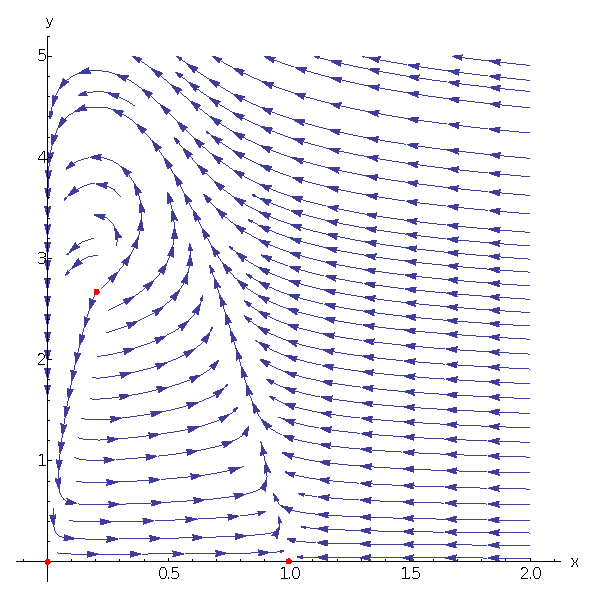
\includegraphics[scale=1.0]{pics/zone1.eps}
\item
В этой области $0 < \gamma < \sqrt{2} - 1$, $\alpha < \frac{4(1 - \gamma)(\gamma + 1)^3}{(\gamma^2+2\gamma-1)^2}$, $D < 0$, $\Tr J(Q) > 0$, то есть $Q$ --- неустойчивый фокус.

Пример с $\alpha = 10$, $\gamma = 0.2$:

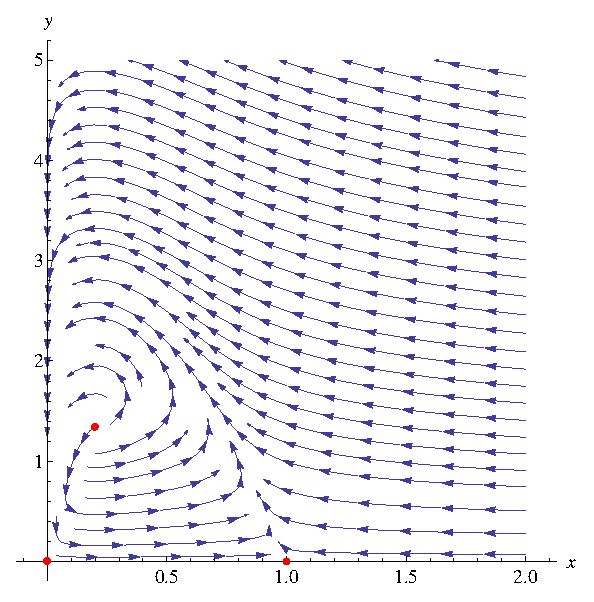
\includegraphics[scale=1.0]{pics/zone2.eps}
\item
В данном случае $\sqrt{2} - 1 < \gamma < 1$, $\alpha < \frac{4(1 - \gamma)(\gamma + 1)^3}{(\gamma^2+2\gamma-1)^2}$, $D < 0$, $\Tr J(Q) < 0$, значит, $Q$ --- устойчивый фокус.

Пример с $\alpha = 5$, $\gamma = 0.5$:

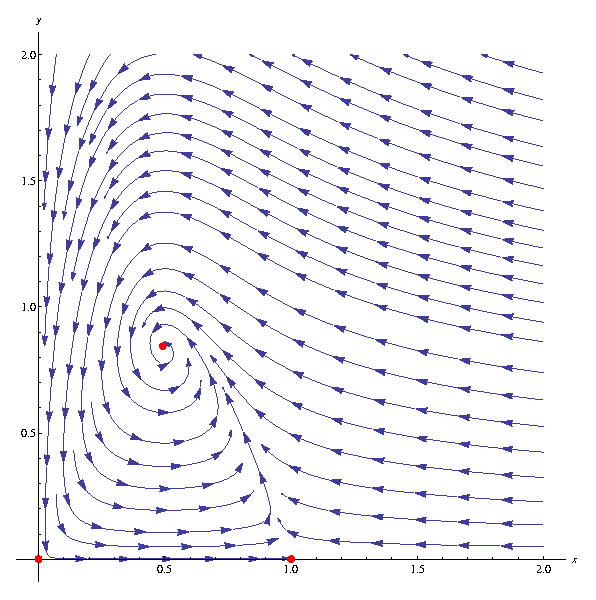
\includegraphics[scale=1.0]{pics/zone3.eps}
\item
В этом случае $\sqrt{2} - 1 < \gamma < 1$, $\alpha > \frac{4(1 - \gamma)(\gamma + 1)^3}{(\gamma^2+2\gamma-1)^2}$, $D > 0$, $\Tr J(Q) < 0$, значит, $Q$ --- устойчивый узел.

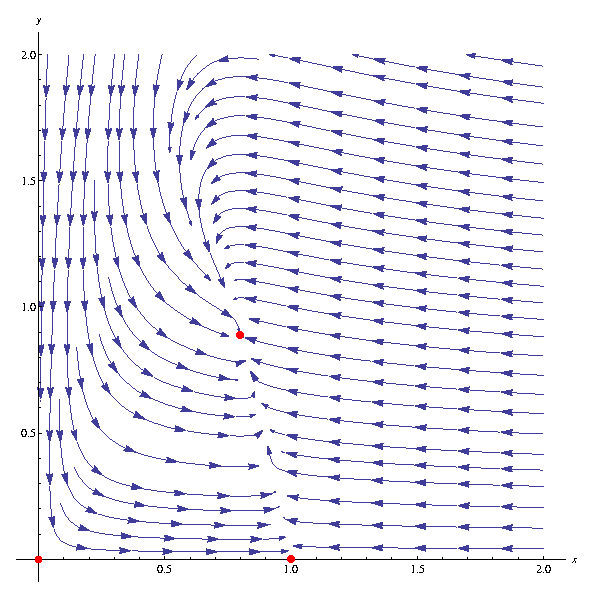
\includegraphics[scale=1.0]{pics/zone4.eps}
\item
В этом случае $\gamma > 1$, то есть точка $Q$ не существует.

Например, $\alpha = 10$, $\gamma = 1.3$:

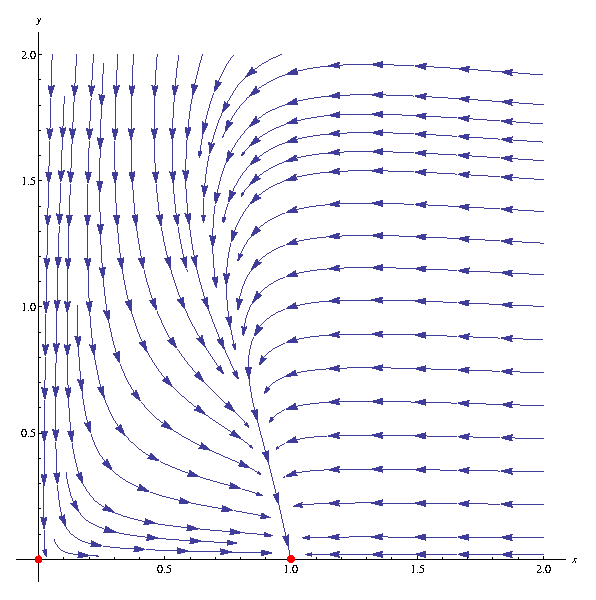
\includegraphics[scale=1.0]{pics/zone5.eps}
\end{enumerate}
\section{Бифуркация Андронова-Хопфа}
\begin{definition}
Бифуркация положения равновесия, соответствующая появлению собственных чисел $\lambda_{1,2} = \pm i \omega_0$, где $\omega_0 > 0$, называется бифуркацией Пуанкаре-Андронова-Хопфа или бифуркацией рождения цикла.
\end{definition}
\begin{theorem}
Любая двумерная однопараметрическая система $\dot{u} = f(u, \alpha)$, имеющая при достаточно малых $\abs{\alpha}$ положение равновесия $u = 0$ с собственными числами $\lambda_{1,2} = \mu(\alpha) \pm i\omega(\alpha)$, $\mu(0) = 0$, $\omega(0) = \omega_0 > 0$ и удовлетворяющая условиям невырожденности
\begin{gather}
\frac{d}{d\alpha}\mu(\alpha) \neq 0, \notag \\
l_1(0) \neq 0,
\end{gather}
где
$$
l_1(0) = \frac{1}{2\omega_0} \Real(ig_{20}(0)g_{11}(0) + \omega_0g_{21}(0)),
$$
в окрестностях начала координат локально топологически эквивалентна одной из двух динамических систем:
\begin{gather}
\dot{v_1} = \alpha v_1 - v_2 + \sgn l_1(0)v_1(v_1^2 + v_2^2),
\dot{v_2} = v_1 - \alpha v_2 + \sgn l_1(0)v_2(v_1^2 + v_2^2).
\end{gather}
\end{theorem}

В исследуемой системе появление чисто мнимых собственных значений возможно только для точки $Q$ при $\gamma = \sqrt{2} - 1$. Следовательно, точка $Q$ имеент координаты $\left( \sqrt{2} - 1, \alpha(\sqrt{2} - 1)^2 \right)$. Матрица Якоби имеет вид:
$$
J(\sqrt{2} - 1, \alpha(\sqrt{2} - 1)^2) = \left[ \begin{array}{ccc}
0 & 1 - \sqrt{2} \\[0.5em]
\alpha(\sqrt{2} - 1)^2 & 0
\end{array} \right].
$$
Эта матрица имеет собственные значения $\lambda_{1,2} = \pm i \sqrt{\alpha(\sqrt{2} - 1)^3}$.

Проверим применимость теоремы 2. Проверим условие
$$
\frac{d}{d\alpha}\mu(\alpha) \neq 0.
$$
Из исследований устойчивости $Q$ следует, что $\mu(\gamma) = \Tr J(Q) = -\frac{\alpha(\gamma^2 + 2\gamma - 1)}{(\gamma + 1)^2}$.
\begin{gather}
\mu(\sqrt{2} - 1) = 0, \notag \\
\frac{d}{d\gamma}\mu(\gamma) = \frac{\alpha(-1 + \gamma(5 + \gamma(3 + \gamma)))}{2(1 + \gamma)^3}, \notag \\
\frac{d}{d\gamma}\mu(\sqrt{2} - 1) = \alpha(\sqrt{2} - 2) \neq 0. \notag
\end{gather}

Найдём собственные векторы матриц $J(Q)$ и $J^T(Q)$, соответствующие собственным значениям $\lambda_1$ и $\lambda_2$:
\begin{gather}
p = \left[ \begin{array}{ccc}
i\frac{1}{\sqrt{\alpha(\sqrt{2} - 1)}} \\[0.5em]
1
\end{array} \right], \notag \\
q = \left[ \begin{array}{ccc}
i\sqrt{\alpha(\sqrt{2} - 1)} \\[0.5em]
1
\end{array} \right]. \notag
\end{gather}

Представим $f(u, \gamma)$ в виде $J(Q)u + F(u, \gamma)$. Нормируем $p$ и $q$ так, чтобы $\scalar{p}{q} = 1$ и $\scalar{\overline{p}}{q] = 0}$, для чего поделим $p$ на $2$. В данном случае $\scalar{p}{q} = \overline{p_1}q_1 + \overline{p_2}q_2$. Для того, чтобы найти первую ляпуновскую величину, введём комплекснозначную функцию:
$$
G(z, \omega) = \scalar{p}{F(zq_1 + \omega\overline{q_1}, zq_2 + \omega\overline{q_2})}.
$$
Вычислим некоторые её частные производные по $z$, $\omega$ при $z = \omega = 0$:
\begin{gather}
g_{20} = G_{zz}, \notag \\
g_{11} = G_{z\omega}, \notag \\
g_{21} = G_{zz\omega}. \notag
\end{gather}

Вычислим ляпуновскую величину по формуле:
$$
l_1(0) = \frac{1}{\omega_0}\Real(ig_{20}(0)g_{11}(0) + \omega_0g_{21}(0)),
$$
где $\omega_0 = \sqrt{\alpha(\sqrt{2} - 1)^3}$, и получим:
$$
l_1(0) = -\frac{1}{4}\frac{\alpha^{3/2}(5\sqrt{2}\alpha - 7\alpha - 3\sqrt{2} + 4)}{(\sqrt(2) - 1)^{3/2}}.
$$

Из полученной формулы следует, что $l_1(0) > 0$ при $\alpha \in \left( 0, \frac{3\sqrt{2} - 4}{5\sqrt{2} - 7} \right)$, и $l_1(0) < 0$ при $\alpha > \frac{3\sqrt{2} - 4}{5\sqrt{2} - 7} \approx 3.414213562373090$. Тогда в зависимости от $\alpha$ бифуркация может иметь различный характер:
\begin{enumerate}
\item
$l_1 > 0$. В этом случае имеет место суперкритическая бифуркация (мягкая) с рождением единственного устойчивого цикла.
\item
В случае $l_1 < 0$ происходит субкритическая бифуркация (жёсткая), то есть система выбрасывается из окарестности неподвижной точки.
\end{enumerate}

Пример возникновения бифуркации ($\alpha = 1$):

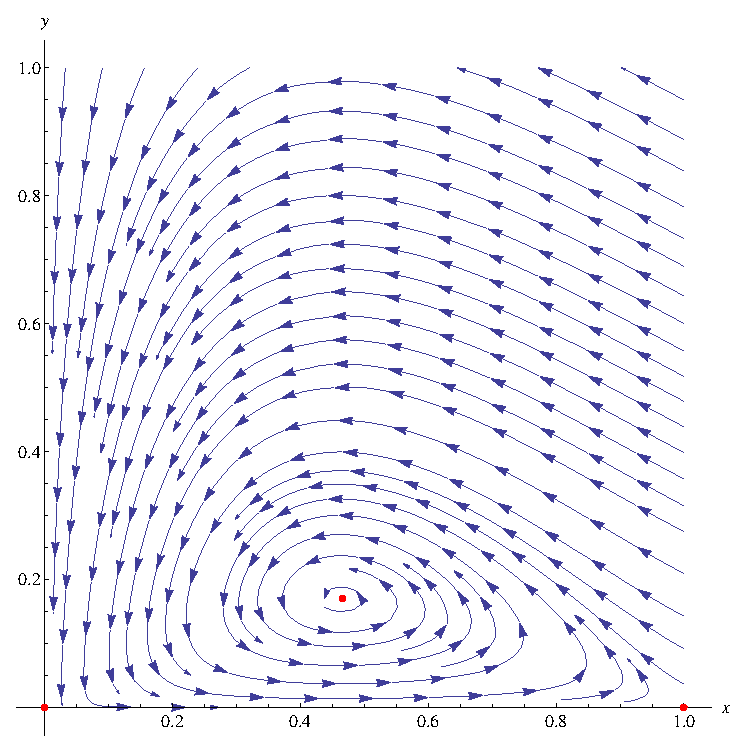
\includegraphics[scale=1.0]{pics/bifur.eps}

\pagebreak
\addcontentsline{toc}{section}{Список литературы}
\begin{thebibliography}{99}
\bibitem{Bratus} Братусь~А.~С., Новожилов~А.~С., Платонов~А.~П. Динамические системы и модели биологии. М.:~Физмалит, 2010.
\end{thebibliography}
\end{document}
